\section{Overview}\label{sec:overview}

\begin{figure}
  \centering
  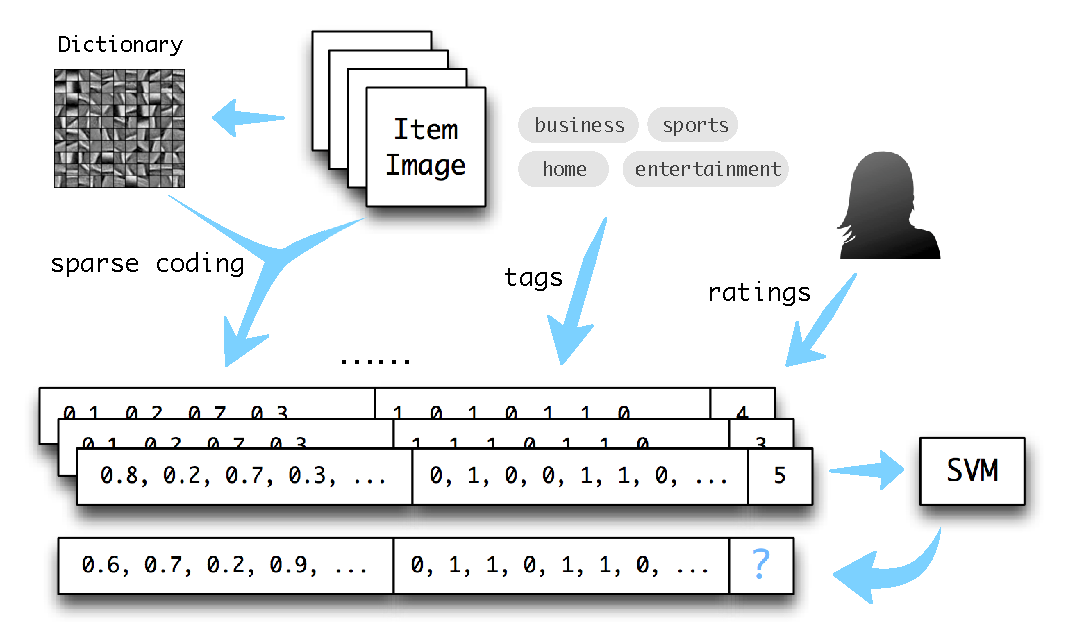
\includegraphics[width=0.9\textwidth]{framework}
  \caption{Framework Overview}
  \label{fig:overview}
\end{figure}

Our framework learned the features of clothing from both the textual labels and the images of clothes on the E-commerce websites. The input of our framework is the user preference which can be modeled from some of the user actions, including browsing time, favorites records, clicking and ratings, etc. The output is the recommended clothes ranked by the possibility that the user would be interested in. There are three major steps in this framework: learn clothing features, model user preference, recommend by rating. Figure \ref{fig:overview} depicts the overall process of personalized recommendation in our framework.

\subsection{Learn clothing features}
There are two features we can leverage to model a garment item. One is textual labels such as cotton for material, sports for style and XL for size, etc. The other is several affiliated images depict each garment. Both the information of textual labels and images will be represented as textual vector and image vector. The representation of textual labels is quite reasonable as we can extract all the possible adjectives like slim, loose, lady and cute in the textual labels. Each adjective represent a feature of the apparel in textual level. If the apparel item contains that feature in its textual label, we can mark 1 in the corresponding place in the textual vector. If not, mark 0. The image processing is more complicated than textual processing to learn the representations. We get the image vector from a base matrix which is also be named as dictionary. The technique details will be discussed in Section \ref{sec:approach}. After both the textual labels and the images being represented as vectors, the two vectors will be combined together by weight as the final representation of each apparel item.

\subsection{Model user preference}
In our framework, each apparel item is corresponded with a preference model for a specific user to map the clothing set to a preference model set of that user. For different users, the map from the clothing set to the corresponding preference set is different. Many actions can be tracked in the E-commerce systems to model the user preference such as scanning time, favorite collection, purchase records and clicks, etc. These features can be modeled as a rating with an approriate range, 1 to 5 for instance. Here we choose the rating to represent the user preference is owing to that the model of user preference has a direct connection with the way how we do recommendation. If we model the user preference with ratings then we can recommend by the predicted ratings of each garment evaluated by machine learning technology. Quantify the user preference is an accurate and easy way to do the recommendation. 

\subsection{Recommend by rating}
The last step of our framework is to recommend clothes which the user has possibility to like and buy it. The ranking strategy of the recommendation is based on the value of possibility evaluated by the machine learning technology which takes the vectors of apparel item and the corresponding ratings of user preference as the input set and the predicted ratings of the chothing whose user preference is unknown. In this step, the major technology we leverage is support vector machine (SVM) which can solve this problem correctly and efficiently. More details can been seen in Section \ref{sec:approach}.\\
\\
In summary, there are three major contributions in this paper and our framework:
\begin{itemize}
	\item We propose a novel and more effective approach to build a framework for personalized apparel recommender systems which focus on the personality of different users and recommend with higher accuracy. We leverage all the possible information of each apparel item from both the textual labels and garment images. We combine the vectors of the two sources together by weight to represent the apparel item. The weight can be adaptive to different users as the emphasis on textual labels and images varied from person to person.
	\item We propose a novel way to leverage the different images affiliated to one apparel item. We treat these images as distinctive garment images with the same textual labels and ratings from its origin apparel. For example, if an apparel item has ID 4 and contains 3 images I1 I2 I3 to dipict this garment as well as a textual label T. If the corresponding preference of this garment has been known from a specific user and the rating is R. Then in our framework we treat these three images affiliated to the same apparel as three distinctive apparel but with the same textual label T and the rating R. This processing can enhance the efficiency of the item model process and the learning process.
	\item We have tried several algorithm that can be applied in our framework.As a consequently we exclude the unsuitalbe ones and leverage the most efficient and suitable algorithms like HAC, K-SVD, SVM, etc.
\end{itemize}
